\documentclass[a4paper]{report}
%\documentclass[a4paper,draft]{report}
 
%PhD Thesis Template for the School of Electronic Engineering and Computer Science, Queen Mary University of London. Stripped from Dan Stowell's PhD.

%BEFORE SUBMISSION DO THESE:
% * deactivate all \includeonly
% * ensure \doneit set to nothing
% * ensure numbering CONTINUOUS from title page on through
% * activate the includes of license, ack, etc
% * check through for question mark errors in render
% * make sure the bibliog doesn't have ugly urls in

\usepackage{graphicx}
\usepackage{ifdraft}
\usepackage{amsmath}
\usepackage{amsfonts}
\usepackage{amssymb}
\usepackage{rotating}
\usepackage{hyperref}
\usepackage{subfig} % apparently subfig is the one to use not subfigure
\usepackage{appendix}
\usepackage{tipa}
\usepackage{clrscode}
\usepackage{setspace}
\usepackage[absolute]{textpos} 
\usepackage[style=numeric]{biblatex}
\addbibresource{refs.bib}
\usepackage{listings}
\usepackage{xcolor}

\setcounter{secnumdepth}{3}

\definecolor{dkgreen}{rgb}{0,0.6,0}
\definecolor{gray}{rgb}{0.5,0.5,0.5}
\definecolor{mauve}{rgb}{0.58,0,0.82}

\lstset{frame=none,
  language=C++,
  aboveskip=1mm,
  belowskip=1mm,
  showstringspaces=false,
  columns=flexible,
  basicstyle={\small\ttfamily},
  numbers=none,
  numberstyle=\tiny\color{gray},
  keywordstyle=\color{blue},
  commentstyle=\color{dkgreen},
  stringstyle=\color{mauve},
  breaklines=true,
  breakatwhitespace=true,
  tabsize=3
}

\usepackage[left=1.2in, right=1.2in]{geometry} % activate for ONSCREEN reading shape AT HOME

\begin{document}

\setlength{\TPHorizModule}{200mm} 
\setlength{\TPVertModule}{100mm} 
\textblockorigin{61mm}{19mm}
\setlength \parindent{0em}
\setlength \parskip{1em}

%%%%% thanks alex mclean for super-useful onscreen reading tip:
%\usepackage[top=0.1in, bottom=0.1in, left=0.3in, right=0.3in, paperwidth=11in, paperheight=7in]{geometry} % activate for ONSCREEN reading shape AT HOME
%\usepackage[top=0.1in, bottom=0.1in, left=0.3in, right=0.3in, paperwidth=11in, paperheight=8.5in]{geometry} % activate for ONSCREEN reading shape AT WORK

\onehalfspace{}

% activate the appropriate shortcut, whether or not to show this in titles
%	\providecommand{\doneit}{DONE: }
%	\providecommand{\doneit}{}

% Some specific notations used:
\providecommand{\OT}[1]{\operatorname{\Theta}\bigl(#1\bigr)}
\providecommand{\OOm}[1]{\operatorname{\Omega}\bigl(#1\bigr)}
%\newcommand{\concat}{{\,++\,}}

% numbering starts from here:
\pagenumbering{arabic}

% titlepage stuff
\title{Parameter automation \\for granular synthesis}
\author{author: Karol Bakunowski \\
\\
supervisor: Michael Zbyszyński\\
\\
BSc (Hons) Music Computing\\
Goldsmiths, University of London
}

\date{2019}

\maketitle
% qmul rules say abstract must be FIRST after title page

\begin{abstract}
My research is about stuff.

It begins with a study of some stuff, and then some other stuff and things.
\end{abstract}  

\renewcommand{\abstractname}{Acknowledgements}
\begin{abstract}
Acknowledge all the things!
\end{abstract}

\include{license}

\tableofcontents
\listoffigures
\listoftables

\include{abbreviations}

\chapter{Introductiones}
% %i should consider writing a 'hook' sentence/paragraph here to draw readers
% %attention and make them interested in the rest of the paper
\section{Aims and Objectives}

The initial aim of the project was to implement a machine learning
solution to the task of granular synthesizer programming based on
sound matching.  Consequently building a tool that would assist
musicians in creating interesting sounds, provided an audio input to
the system.

Throughout the entire development process, the focus remained mainly
on creating a well functioning, usable program, despite some
shortcomings in the areas of synthesis, audio analysis and machine
learning respectively. Integrating these three modules well took
priority over designing a more sophisticated solutions to each
individual problem. Consequently allowing for creation of a tool
functioning in near real-time, with the possibility of extending the
modules that contribute to the whole.

The methods here differ from other approaches in literature (cite some
papers that have done this, eg. Matthew, Leon) primarily in that here,
one standalone tool has been created, that is usable on it's
own. Users have direct ability to program the synthesizer using input
from the microphone, and the entire process is handled by two
buttons. No prior experience with programming is required, and the
only assumption made about the user is knowledge of basic synthesizer
programming.

The main objectives therefore are:

1. To build a tool that is helpful to artists in the process of
creating sounds 

2. To challenge the interaction between an artist and a preset as a
starting point to synthesis 

3. To achieve a response that is not only stimulating to the user but
also differs from simply randomizing the parameter values

In measuring the project's success, the subjective sonic coherence and
similarity of predicted outputs may be considered the best indicator (the
human discriminator?). Undoubtedly, if the predictions achieved are
satisfying to the user, the main goal of this project was
achieved. Additionally, users' opinions about whether the tool would
be usefull in their work process will be a good indicator of the
project's success.

Along with that, a quantitative analysis, such as comparing the audio
descriptors on target and predicted sounds should prove itself useful.
It will allow to do a quite generalisable, and objective comparison of
target vs. predicted sounds. This process will enable the evaluation
of neural networks used for predicting the parameter values, and help
in assuming whether users will find the program useful.  

EDIT!!!!!!:
In (future chapters) I provide some critique on established techniques of
assessment of these types of problems and ultimately conclude that some stuff in
the best way of doing it.

\subsection{Deliverables}

In the inerest of achieving the above decalred goals, I propose a
standalone program, that allows users to set parameters of a granular
synthesizer based on a one second buffer of audio, generated form the
microphone input.

The program could be arbitrarily split into three different modules,
in order to clarify the it's basic structure. Namely, synthesis, audio
analysis and machine learning.

The synthesis is implemented in the ``Juce'' framework. Audio analysis
tools from the ``Essentia'' library are used to help create training
datasets, as well as help make predictions. And lastly, an
implementation of a Multilayered Perceptron feedforward neural network
with the ``Keras'' API is presented. The ``Frugally Deep'' library is
responsible for deploying the ``Keras'' model into C++ code, allowing
for near-real time performance, and removing the need for
communication between C++ and Python. 

Resulting program is a standalone ``JUCE'' application, capable of
performing granluar synthesis, extracting audio features, and
predicting parameter values of the synthesiser based on microphone
input.

% \cite{example-citation} Some more things. 
% Inline citation: \bibentry{example-citation}

%This section should be about 500 words.
%
%You can't write a good introduction until you know what the body of
%the paper says. Consider writing the introductory section (s) after you have completed the rest of the paper, rather than before.
%
%Be sure to include a hook at the beginning of the introduction. This is a statement of something sufficiently interesting to motivate your reader to read the rest of the paper, it is an important/interesting scientific problem that your paper either solves or addresses. You should draw the reader in and make them want to read the rest of the paper.
%
%The next paragraphs in the introduction should cite previous research in this area. It should cite those who had the idea or ideas first, and should also cite those who have done the most recent and relevant work. You should then go on to explain why more work was necessary (your work, of course.)
% 
%What else belongs in the introductory section (s) of your paper? 
%
%1.    A statement of the goal of the paper: why the study was undertaken, or why the paper was written. Do not repeat the abstract. 
%
%2.   Sufficient background information to allow the reader to understand the context and significance of the question you are trying to address. 
%
%3. Proper acknowledgement of the previous work on which you are building.
%Sufficient references such that a reader could, by going to the library, achieve
%a sophisticated understanding of the context and significance of the question.
%
%4.    The introduction should be focused on the thesis question(s).  All cited work should be directly relevant to the goals of the thesis.  This is not a place to summarize everything you have ever read on a subject.
%
%5.    Explain the scope of your work, what will and will not be included. 
%
%6.    A verbal `road map' or verbal `table of contents' guiding the reader to what lies ahead. 
%
%7.    Is it obvious where introductory material (`old stuff') ends and your contribution (`new stuff') begins? 
%
%Remember that this is not a review paper. We are looking for original work and interpretation/analysis by you. Break up the introduction section into logical segments by using subheads. 

%%% Local Variables:
%%% mode: latex
%%% TeX-master: "dissertation"
%%% End:


\chapter{Literature Review}
\label{chap:lit}

\section{Problem background}

\subsection{Synthesizer programming}

Programming synthesizers can be enjoyable, fun and gratifying, yet
very often presents a big challenge. The amount of adjustable
parameters on such a device can be overwhelming, and consequently the
range of sounds that can be achieved is usually very extensive.

Granulation, or any other corpus based synthesis technique for that
matter, presents what could be called a special case in this
domain. Not only do the parameters determine the final output, but
also the input sample has a tremendous influence over the sound.

In a granular synthesizer, users are presented with choices ranging
from determining the audio to be sampled, to the amliptude envelope
for each grain. A huge array of possibilities.

Therefore the ability to make decisions about programming a granulator
to achieve desired results has to come from either a place of
certainty about what each parameter is responsible for combined with
intuition about the instrument, or a place of experimental though, and
somewhat random parameter value assignments.

Users fairly new in the realm of synthesizer programming may encounter
issues creating sounds they desire. This is to be expected, as like in
any other area, novices have to get through a rather steep learning
curve, to achieve certain intuition, and skill. This, however, often
prevents people from creating what they want, or makes them settle for
less, consequently limiting their creative output.

On the other hand, experienced musicians are constantly looking for
inspiration and new ways of interaction with the process of creating
exciting sounds\cite{herbert_manifesto_2011}. Furthermore, programming
synthesizers by following a not clearly defined intuition, combined
with the use of presets and a mixture of experimantal methods is a
popular approach\cite{noauthor_oneohtrix_2016}, especially considering
the amount of tools available today, and the ease of acquiring
them. The fact of having too many VST plugins in a DAW, is a common
problem today.

There are of course all the people in between the complete novice,
and succesfull artist. They may have some experience, and can follow
their own intuition, yet are trying to find their own sound, and
define their style of production. Making that process easier,
consequently making the music making process more accessible would be
a great contribution to the community (EDIT, BUT IDEA IS GOOD).

\subsection{Sound matching}

The problem of sound matching seems to be almost unexistent for
humans. We are able to hum along a song we have heard previously, or
replicate sounds of different objects, like cars, or animals, like
dogs. This activity does not present any real challenge for us. It
could even be said that such a behaviour is taken for
granted.

It has been around since forever, and it is mostly how children learn
language. The word ``onomatopoeia'' desribes a process of creating a
word that phonetically resembles, or suggests the sound it describes
(SOURCE) and has been around even before language came aobut (CHANGE)
(ADD SOURCE)!

Conversly, creating a specific desired sound on an instrument of any
kind takes serious practice, and sacrifices. Musicians who are able to
translate what they hear in their head, directly to an instrument, be
it a physical one like piano or guitar, or a software based
instrument, are considered viruosic. Therefore, the ability to
replicate any sound in a synthesizer, based solely on an audio input
seems like a very intuitive way of interaction, and possibly an
inspiring way of working for musicians.Additionally, it would blur the
line between a begginer, and a virtuoso in that specific area,
allowing people with less technical expertise to create music they
want to hear.Primarily, however, such interaction would be an immensly
helpful, and time-saving scenario for musicians, allowing them to
spend more time on creative work, taking over, at least partially the
task of programming a synthesiser.

In the next three sections I go over each area of the project, and talk
about previous work that has been done on each aspect.

\section{Audio descriptors}

Because of the way audio is represented digitally, mimicking
sounds is not as intuitive for computers as it is for
humans. Algorithms that are capable of generating meaningful data
about given audio signal are needed in order to describe sounds in
different ways, and based on different assumptions. (add more about
why these are needed, and pure audio singal can't be used?)

A great amount of these analysis tools exist, and a lot of them are
easily accessible either through libraries in different programming
languages, such as `libriosa'\cite{noauthor_librosa_nodate} for
Python, or `Essentia'\cite{noauthor_homepage_nodate} for C++, or
directly through different audio software such as
`Audacity'\cite{noauthor_audacity_nodate} or most Digital Audio
Workstations today.

The decision about which were suitable for the task of automatic
synthesizer programming was mainly based on previous research done in
this domain. However, some amount of experimentation with different
audio extractors was done, to see if certain assumptions made during
early stages of the project were correct.

EXPAND:
The early work done with focus on sound matching was using mainly
spectral features, such as the Fast Fourier Transform (source). More
recently, however, the Mel-frequency Cepstrum Coefficients seem to be
the prefferable descriptor (source) [22][23]

\subsection{Mel-frequency Cepstrum Coefficients}

In order to get information about the frequencies present in an audio
signal, a conversion to the frequency domain has to be
done. Extracting frequency information form the time-domain can be
done (reference), however a well established, and more prefferable
method today exists, which is the Fourier Transform (source). The
algorithm can dissect a signal to it's most basic sinusoidal
components, therefore determining how much of which frequencies are
present in the signal allowing for creation of a spectrogram.

The Fourier Transform, or more precisely it's less computationally
expensive version the fast Fourier Transform (FFT) (source) serves as
the basis to compute an algorithm which is possibly the most powerful
algorithm for determining the timbre of an audio signal today - the
Mel-frequency cepstrum coefficients (MFCC).

Details of this algorithm are well beyond the scope of this paper,
however many studies have been done to prove the usefullness of MFCCs
in sound matching
tasks\cite{yee-king_synthbot:_nodate}\cite{heise_automated_2009}, as
well as in monophonic instrument recognition
tasks\cite{eronen_comparison_2001}.

(not sure if this paragraph is needed?)
Today they are mainly used in speech symthesis and speech recognition,
however can be apply to any signal, and are a very powerful
descriptor. More recently MFCCs have been used in the field of music
information retrieval applications (sources)

Blurring the line between timbre and rhythm detection, a sequence of
MFCCs can tell a computer quite a substantial amount of information
about rhythmical qualities of sound, as well as any temporal changes
in both time, and frequency domains. Listener studies have shown that
movement in MFCC space is associated with a similar `sized' movement
in human perceived timbre space\cite{terasawa_center_2005} (change as this sentence is a total ripoff)

\subsection{Spectral Flux}
MORE CONTENT, CITE PAPERS (not specifically used for sound matching
tasks i think)

Onset detection, which tries to estimate how many `peaks' there are
in a signal is a very useful algorithm to estimate how much rhythmical
content there is present.

It can be achieved with an algorithm called ``Spectral Flux''. It
compares consequtive spectra, determining how much change has happend,
producing a float value corresponding to it. By thresholding this
change, based on the mean value of the flux, floats corresponding to
the onsets in a signal can be derived (source, source).

\section{Synthesis}

Research has been done previously as an investigation into automation
of parameters in synthesizers based on sound matching. Taking a
snippet of sound, the algorithm would try to find parameter settings
to match a produced sound as closely as possible to the
source\cite{yee-king_automatic_2018}.

This research mostly focuses on FM
synthesis\cite{horner_machine_1993}, although experiments on different
synthesis techniques have been done\cite{dahlstedt_creating_nodate},
including VST plug-ins\cite{yee-king_synthbot:_nodate}.

However, using this approach on corpus-based synthesis remains an
untapped area of research, worth
investigating\cite{mcdonald_neural_2017}.

Many software based granular synthesizers exist, both in standalone
(source, source) and VST form (sources). The implementations, and
certain parameters etc. differ in each example. Nonetheless, this type
of synthesis introduces an interesting problem in the contex of
parameter prediction, which applies to any corpus based synthesis
engine. The sounds created are heavily based on the sample fed into
the synthesizer. Each parameter changes meaning significantly, once
the input sample is changed. 

Two possible solutions come to mind, when trying to overcome this
problem. Using one input sample for synthesis, and trying
to predict samples for one perticular instance of the granulator is one.
Another, would be trying to fit some universal analysis algorithms,
that could decribe rhythym, pitch, density of sound etc. independently
of the original sample. This way any sample could be `molded' into
what would resemble the original prediction target. 

Concatenative synthesis is an alternative approach to this problem. It
could be beneficial, as it would try to find `grains' as closely
resembling parts of the target as possible, and recreate it using
little parts, almost like puzzles, that the algorithm thinks
fit. However, that approach also has limitations, as it could only
recreate the target sound out of the samples stored in it's database,
therefore making the output biased. (cataRT source)

\section{Predictions}

A impressively sized bulk of work has been done around the automatic
programming of synthesizers. Possibly the most complete body of work
on the topic is Yee-King's thesis
\cite{yee-king_automatic_nodate}. One of the first approaches
described by Horner et al. was a Genetic Algorithms \cite{horner_machine_1993}
aimed at predicting settings for an FM synthesizer. Another
possibility would be to use the simplest algorithms available and
suitable for this task, the Hill Climber algorithm (source-matthew's
paper).

These approaches are all quite valid, however the main problem
occuring with them is the computational time required to come up with
a result. None of these approaches really offers the ability of
prediction in real, or near real time, making them an unappealing
choice for user facing systems.

An approach in line with the most recent reaserach would seem to be an
adaptation of neural networks for the task of automatic synthesizer
programming. Fedden et. al (source) has made a vst host for extraction
of parameters, and creation of a dataset, as well as a framework to
train neural networks in. (more?) A more in depth exploartion of
possibilities in this domain was done by Yee-King, Fedden, and
D'Inverno et al (source), which compared and considered GA, HC, MLP,
LSTM, and LSTM++ algorithms.

Another possibility is the use of convolutional networks, however this
approach would be limited to classification.

Alternatively, in order to try and generalise the predictions for
different input samples for the synthesizer. The predictions could be
devided between different parameters. Then linking different
prediction algorithms with different parameters could possibly allow
for a creation of a more direct relationship between audio descriptors
and the synthesis results. No widely available research seems to
approach this task in this modular way, yet it seems like discovering
certain linear relationships between parameter values and audio
descriptors is certainly possible.

%stick to this shit over here:
It seems that most of this research focuses on reproducing the
original input\cite{tatar_automatic_2016}. Perhaps more interesting
and novel sounds could arise as an effect of bad performance, but is
does not seem to be the desired outcome in most cases.

%% advice 

%The next paragraphs in the introduction should cite previous research in this
%area. It should cite those who had the idea or ideas first, and should also cite
%those who have done the most recent and relevant work. You should then go on to
%explain why more work was necessary (your work, of course.)

%Sufficient background information to allow the reader to understand the context
%and significance of the question you are trying to address.

%Proper acknowledgement of the previous work on which you are building.
%Sufficient references such that a reader could, by going to the library, achieve
%a sophisticated understanding of the context and significance of the question.

%The introduction should be focused on the thesis question(s). All cited work
%should be directly relevant to the goals of the thesis. This is not a place to
%summarize everything you have ever read on a subject.

%%% Local Variables:
%%% mode: latex
%%% TeX-master: "dissertation"
%%% End:


\chapter{Methods}
\label{chap:meth}

The general approach to solving the problem of automatic synthesizer
programming is based on prior work done in this domain. The basic
structure could be described like so:

\begin{figure}[h]
\caption{Program flow}
\centering
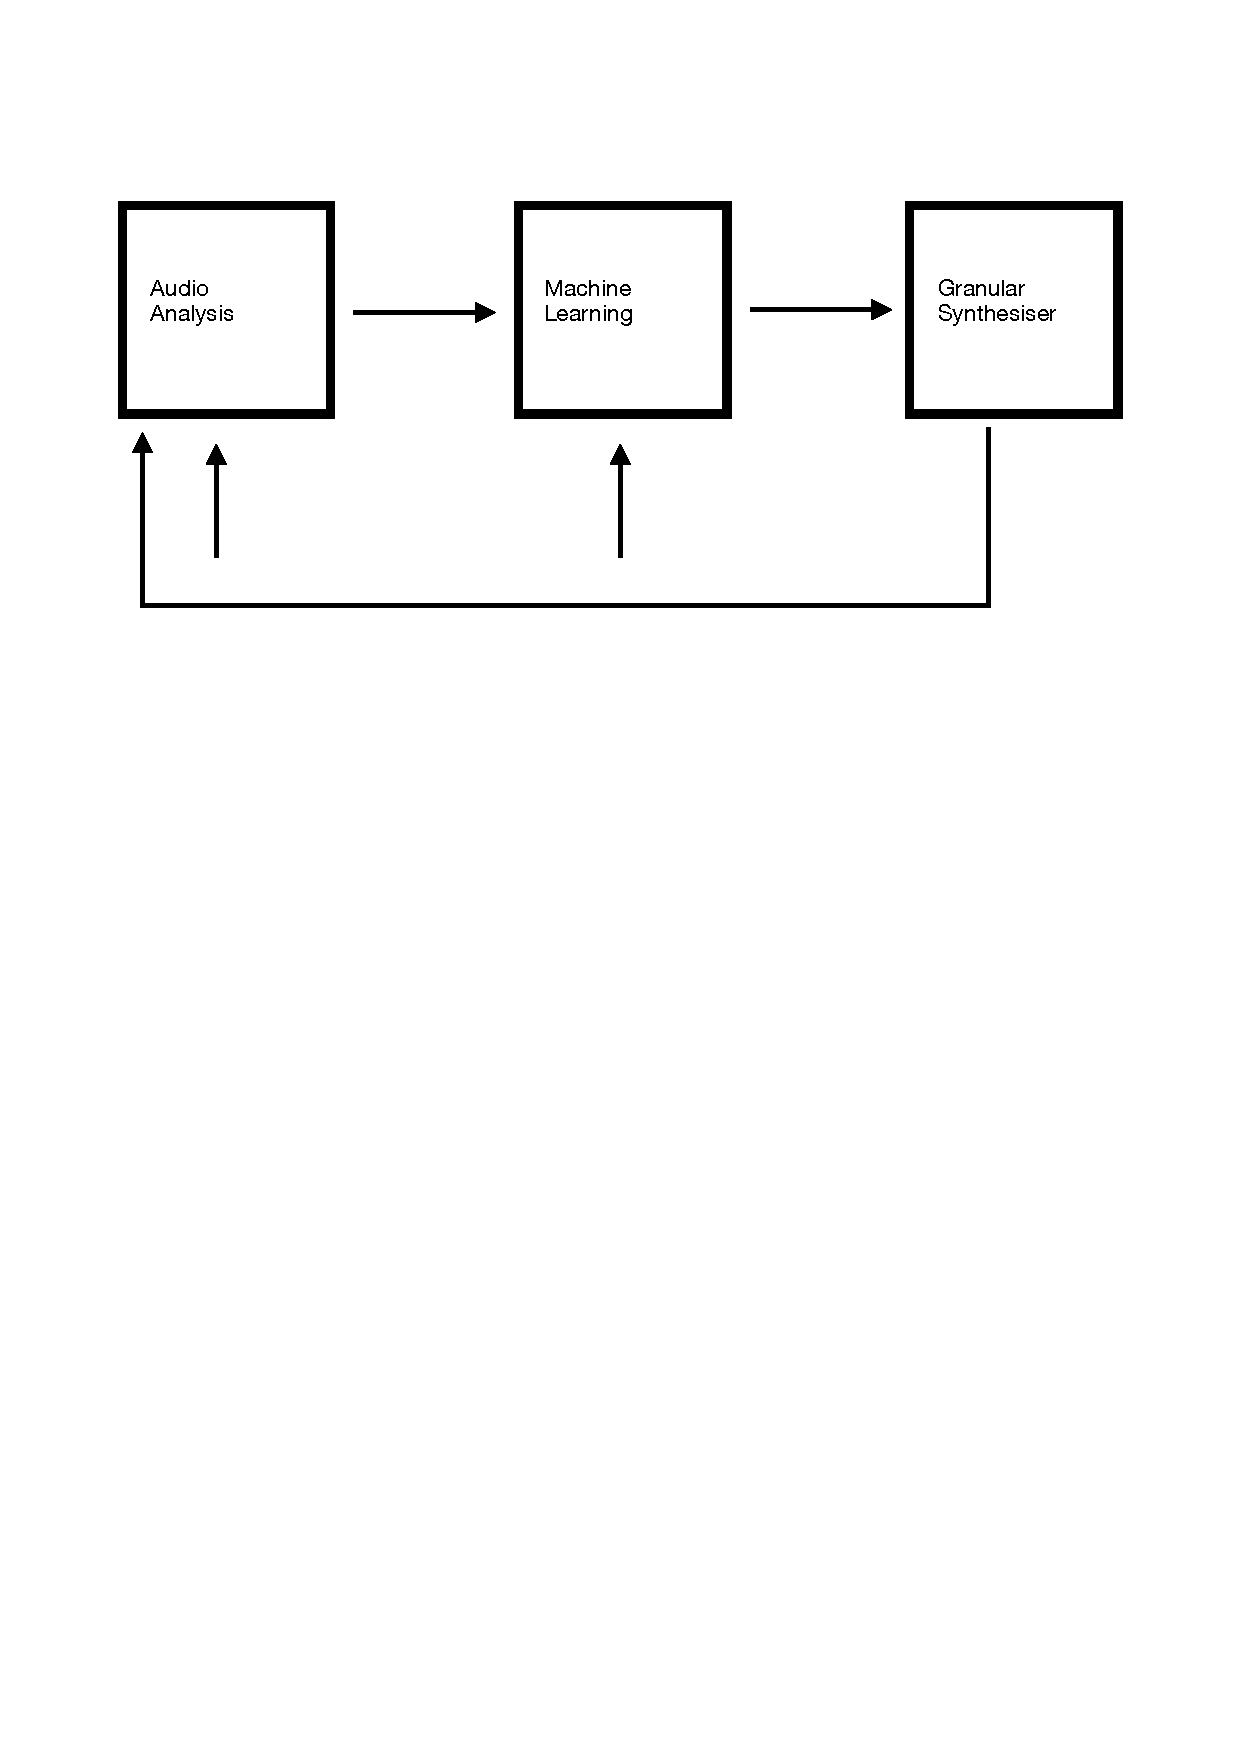
\includegraphics[width=0.5\textwidth]{images/flowchart}
\end{figure}

The box ``Granular Synthesiser'' in figure 3.1 represents the synthesis
engine. It was implemented in C++, using the `JUCE' framework
(SOURCE).

``Machine Learning'' stands for the predictions module, or more
precisely the Multilayer Perceptron model built in ``Keras'', and
later ported to C++ with the help of the ``Frugally Deep'' library.

The ``Audio Analysis'' square represents the aspect of the
project responsible for extracting audio features from input
sounds. This was done with the ``Essentia'' library, that allowed me
to perform frame cutting, windowing, extracting the spectrum and
finally MFCCs on any specified buffer.

Lastly, the ``Audio Input'' represents the microphone input, which is then
analysed, and predictions are made on those values, in order to set
parameters of the synthesizer.

\section{Audio descriptors}

%check if statement correct near source:
The decision about which audio feature extraction algorithms were used
was mainly based on previous research done in this domain. As
mentioned in \autoref{chap:lit} the MFCC algorithm is proven to be one
of the most reliable desriptors available, and can not only describe
the temporal qualities, but also be indicative of the changes that
happen in the input signal\cite{terasawa_center_2005}.

Great results, and the easiness of quantative evaluation of the
MFCC\cite{yee-king_automatic_2018} were the main factors, outweighing
different, potentially usefull feature extractors.

Based on that, it is the only algorithm used in the final version of
the program, and further justifications of that decision are provided
later in this chapter.

However, some amount of experimentation with different feature
extractors was done, in order to see if certain assumptions made during early stages of the project were
correct. Mainly, if certain descriptors could be used in direct
correlation to different parameters of the synthesizer. Such as
frequency content with ``pitch'' parameter, or rhythmical content with
the the size of the grains.

\subsection{Mel-frequency Cepstrum Coefficients}

The validity of MFCC for musical applications was established in
(CHAPTER 2). Below, I detail how the algorithm is computed generally,
and provide my implementation in parallel to the explenation.

The spectrum, or a representaion of a signal in the frequency domain
serves as a foundation for the MFCC algorithm. Conversion of a
signal from time to frequency domain, can be done with the Fourier
Transform algorithm. It can dissect a signal to it's most basic
sinusoidal components, therefore determinig how much of which
frequencies are present in the signal, allowing for the creation of a
spectrogram.
% Extracting frequency information form the time-domain can be
% done (reference)

The spectrum is calculated by performing the Fourier Transform on a
windowed frame of a signal. (source, what if we took mfccs on the
entire song lol?) Once that spectrum is computed, it's powers are
mapped into the mel scale, using triangular overlapping windows. Next,
logs of the powers at each of the mel frequencies is taken, creating a
list of these values. Then, the discrete cosine transform of that list
is computed. The MFCC are the ampliduted of the resulting spectrum.

To summarize, the Mel-frequency cepstrum is a representaion of the
short-term power spectrum of sound, based on a linear cosine transform
of a log power spectrum on a nonlinear mel scale of frequency (WTF,
CHANGE AND ADD SOME REFERENCE TO THE DESCRIPTION). In turn, the MFCC,
are coefficients that collectively make up the Mel Cepstrum.

%The MFCCs are commonly derived as follows:
%
%\begin{enumerate}
%\item{Take the Fourier Transform of a signal}
%\item{Map the powers of the spectrum obtained into the mel scale,
%    using triangular overlapping windows}
%\item{Take the logs of the powers at each of the mel frequencies}
%\item{Take the discrete cosine transform of the list of mel log
%    powers, as if it were a signal}
%  \item{The MFCCs are the amplitudes of the resulting spectrum}
%\end{enumerate}

There can be variations on this process, such as differences in the
shape or spacing of the windows used to map the scale, or addition of
dynamics features such as delta and deltadelta coefficients.(ADD
SOURCE AND CHANGE - total ripoff)

The biggest advantage of this algorithm is that in the MFC the
frequencies are spaced in a way which approximates the human auditory
system more closely than the cepstrum used in a Fourier Transform.

% %work on this, do a better job of explaining
% The process decribed above was achieved with algorithms provided by
% the `Essentia' library\cite{noauthor_homepage_nodate}. It works in a
% modular way, that can roughly be described as spiltting the algorithms
% into lower, and higher level algorithms. They can be then `stacked' to
% create more complex chains of computation, capable of extracting, as
% in this case, the MFCCs. The algorithms have to be defined beforehand,
% with an input as well as output for each of them.

Access to this algorithm is relatively easy, when using Essentia,
because of it's high level API. It allows for arranging algorithms in
a sequence, and connecting them with share inputs and
outputs. Therefore, to compute the MFCC in Essentia, one has to first
compute the spectrum, and it's output serves as an input to the MFCC
algorithm, that computes the process described above.

The buffer on which MFCC are calculated is created in the following manner:
sratatatatata
\begin{lstlisting}

// computing the essentia algorithms
if (audioFeatureExtraction.playbackBuffer.index < audioFeatureExtraction.getLengthOfBuffer())
{
    const auto* channelData = bufferToFill.buffer->getWritePointer(0, bufferToFill.startSample);
    for (auto i = 0; i < bufferToFill.numSamples; ++i)
    {
        audioFeatureExtraction.pushNextSampleIntoEssentiaArray(channelData[i]);
    }
}
else
{
    //randomParameterWalkthrough();
}

\end{lstlisting}

% perhaps add sources here
The Fourier Transform is computed on frames of the signal, making
the assumption that what is inside of that frame is a single period of
repeating waveform. Most sounds are ``locally stationary'', meaning
that over a short period of time they really do look like a regularily
repeating function, which approximates enough for the Fourier
Transform to work. It leads, however, to a situation where the
endpoints of each frame are discontinuous, creating ``spectral
leakage''. In an effort to reduce this effect, the technique known as
overlapping is applied. The consequtive frames are overlapped by a
certain amount of samples known as ``hopsize''. This allows for taking
an average of multiple overlapping frames, and consequently a better
representation of the time domain signal.

Lengths of both the frames, and the size of the hopsize vary, and
depend on application. However the standard values are assumed to be
2048 samples and 1024 samples consequtively.

Here is how the frames, windowing, and overlapping are implemented
using Essentia:

% code
% description

The process of computing that is as follows:

\begin{itemize}
\item Firstly, an audio buffer on which the computation will be
  performed has to be specified. Here, one second of sound is written
  into a buffer (C++ vector), that then gets passed to the first algorithm
\item `FrameCutter' is where the buffer first arrives. This function
  splits the buffer into multiple frames, as dictated by the
  parameters. Then, each frame, separately is sent further down the
  chain, with the help of a while loop
\item Each consequtive frame of the buffer arrives at the `Windowing'
  algorithm, which essentialy smoothes out the edges of each frame.
\item Once the windowing is applied to the frame, the spectrum of the
  input signal is calculated.
\item Finally, the Mel-Frequency Cepstrum Coefficients are calculated
  for the frame
\end{itemize}

\begin{figure}[h]
\caption{logic of the MFCC computation}
\centering
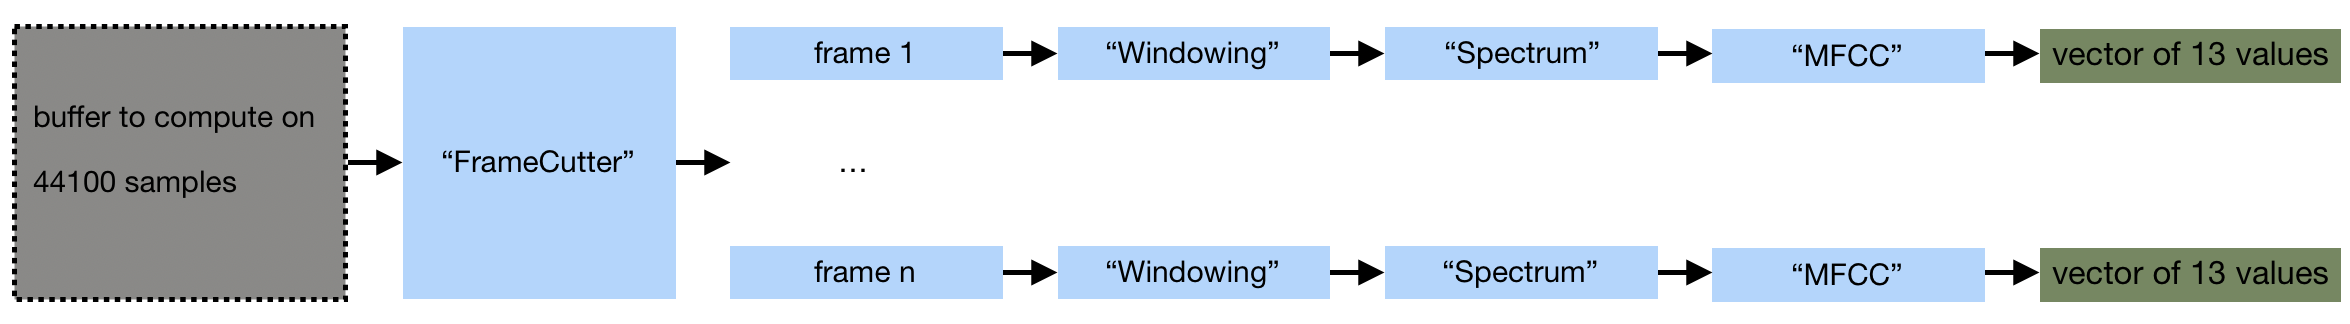
\includegraphics[width=1\textwidth]{images/essentia_logic}
\end{figure}



% this goes below descriptions of each thing, and it's code
% implementation first.
Let's assume we are trying to analyse audio input which is 10 seconds
long. First, we have to split the signal into an appropriate amount of
frames on which the Fourier Transform will be calculated. Each of
these frames will be windowed, and overlapped.

With the values stated above our input would be split into frames of
size 2048 (approximately x ms.), each frame 1024 samples further than
the previous one.

For each frame, MFCC are calculated based on the extracted FFTs, as
described above. The result for one frame is a vector of 13 floating
point values, each corresponding to a different range of
frequencies. (talk about why 13, because default essentia values?)

At a sampling rate of 44.1kHz, and a buffer size of 512 samples, this
corresponds to exactly 45 vectors of 13 float values for one second of
sound. Meaning that our hypothetical sound of length of 10 second
would comporomise of 450 MFCCs.

Figure 3.2 in C++ code:
\begin{lstlisting}
void AudioFeatureExtraction::computeEssentia()
{
    while (true)
    {
      frameCutter->compute();

      if (!frame.size())
      {
          break;
      }
      if (isSilent(frame)) continue;
        
      windowing->compute();
      spectrum->compute();
      mfcc->compute();
      
      pool.add("lowlevel.mfcc", mfccCoeffs);
    }
    mergePool.merge(pool, "append");
}
\end{lstlisting}

This process is repeated for each frame, which at the sampling rate of
44.1kHz, and a buffer size of 512 samples, with frame size of 1024,
and hopsize of 512 samples equals to exactly 45 frames per
second. 

As seen above, the results of the computation are written into
``Essentia's'' pool datastructure. Which in turn is written into a
JSON file after a specified interval.

The process for audio feature exraction for input differs slightly,
mainly in that the different algorithms with different inputs and
outputs are defined and go through different functions.

% only include this and section for it in the implementation if not
% enough words
\subsection{Spectral Flux}
% find place for this:
Several different audio features have been experimented with,
especially in the quest of finding universal ones, that could be
applied to any source file in the granular synthesizer. One of such
features is onset detection. It's implementation consists of the
spectral flux algorithm, thresholding and peak finding, in order to
estimate how many peaks, or onsets are in a specified buffer. (more
description, or is this useless to talk about?)

However, during testing, which is described in chapter 4, such a
connection was not found, therefore this project solely depends on MFCCs.
%
MORE CONTENT, CITE PAPERS (not specifically used for sound matching
tasks i think)
In an effort to explore different algorithms, and the idea of
assigning one feature to one parameter, exploration into the
onset detection was done.
Onset detection, which tries to estimate how many `peaks' there are
in a signal is a very useful algorithm to estimate how much rhythmical
content there is present.

It can be achieved with an algorithm called ``Spectral Flux''. It
compares consequtive spectra, determining how much change has happend,
producing a float value corresponding to it. By thresholding this
change, based on the mean value of the flux, floats corresponding to
the onsets in a signal can be derived (source, source).

\section{Predictions}
\subsubsection{Definitions and Formulations}
% everything done on one sample only -> here?
One of the main implicit requirements for this project is the ability
to predict parameters in real, or near-real time, considering it is a
user facing program. Literature shows that currently the best way of
achieving that is through neural
networks\cite{yee-king_automatic_2018}. As mentioned in (CHAPTER 2),
they take a considerable amount of time to be trained. Yet, once
trained they can compute results in near real-time. Based on this
assumption, neural networks were the only optimization algorithm used
in this project.

Alternatively, in order to try and generalise the predictions for
different input samples for the synthesizer, instead of just one the
predictions could have been devided between different parameters. This
approach should allow for creation of mappings between different
parameters and audio descriptors. However, due to the fact, that no
correlation was found between spectral flux and grian size parameter,
possibly the most obvious bet at the beggining of the project, this
concept was dropped. Additionally, I was not able to find any
literature that would suggest such correlations. Therfore, and ``easy
route'' was taken in order to achieve results quicker, in the spirit
of achieving one fo the main goals for the project - to build a tool
capable of parameter prediction in real time. Using an already
established technique as suggested by Yee-King et al.

A neccessary step for training any neural network is the creation of a
dataset, linking labels, in this case the MFCC vectors, with features
to be predicted, in this case parameters of the granular synthesizer.

First, I detail how the dataset was created, and it's
implementation. Then I summarize the nature of neural networks
created, as well as their implementation.

\subsection{Dataset}

Initially, I have set out to create a dataset of every possible
combination of parameter values, and their corresponding MFCCs. The
synthesizer would play for one second, the MFCC of that second would
be taken, and parameters would be incremented. I decided that each
parameter would be incremented by a tenth of it's value, for each
iteration, based purely on intuition that this would provide enough
data.

However, even though there are only 5 adjustable parameters, this
process would have taken more than 1000 hours (ca. 41 days) to create
the dataset. It is certainly possible to complete such a process, yet
seemed like an unneccesary step, especially considering that the
performance of neural networks was not known at this point.

% (source here, where did i get the idea?)
Consequently, a different approach was taken. Instead of incrementing
the parameters, a random value was assigned to each, after every
iteration. The random number was always between the unique minimum and
maximum of each parameter.

This was done inside of the C++ JUCE synthesis code. A function
responsible for setting a random value for the parameters was
implemented using the JUCE::Random class. Every second, after each
iteration, the class instance is outputting a random value between
specified ranges, unique for each parameter. This results in
independent changes. It is a pseudorandom number generator, for which
seed was not specified, in order to get different values, if multiple
datasets were desired:

\begin{lstlisting}
void MainComponent::randomParameterWalkthrough()
{
    
    int numOfSamples = 10000;
    Random rand = Random();
  
    audioFeatureExtraction.computeEssentia();
  
    audioFeatureExtraction.paramPool.add("parameters.position", audioFeatureExtraction.count);
    audioFeatureExtraction.paramPool.add("parameters.duration", audioFeatureExtraction.duration);
    audioFeatureExtraction.paramPool.add("parameters.spread", grainStream.filePositionOffset);
    audioFeatureExtraction.paramPool.add("parameters.numberOfGrains", audioFeatureExtraction.streamSize);
    audioFeatureExtraction.paramPool.add("parameters.pitch", grainStream.pitchOffsetForOneGrain);
    audioFeatureExtraction.mergePoolParams.merge(audioFeatureExtraction.paramPool, "append");
  
    audioFeatureExtraction.clearBufferAndPool();
    
    audioFeatureExtraction.count = rand.nextInt(Range<int>(1, grainStream.getFileSize()));
    grainStream.setFilePosition(audioFeatureExtraction.count);
    audioFeatureExtraction.duration = rand.nextInt(Range<int>(10, 1000));
    grainStream.setDuration(audioFeatureExtraction.duration);
    grainStream.filePositionOffset = rand.nextInt(Range<int>(0, 50000));
    audioFeatureExtraction.streamSize = rand.nextInt(Range<int>(1, 10));
    grainStream.setStreamSize(audioFeatureExtraction.streamSize);
    grainStream.pitchOffsetForOneGrain = rand.nextInt(Range<int>(-12, 12));
    
    audioFeatureExtraction.count2 += 1;
    cout << "round:" << "/t" << audioFeatureExtraction.count2 << endl;
  
    if (audioFeatureExtraction.count2 == numOfSamples)
    {
        audioFeatureExtraction.mergedMFCCs->compute();
        audioFeatureExtraction.mergedParameters->compute();
        changeState(TransportState::stopping);
    }
}
\end{lstlisting}

After each iteration, the MFCCs are computed, and added to the
dataset. Then parameter values are added to the dataset. Next, the
temporary vectors holding the values, as well as all of the Essentia
algorithm's inputs and outputs, and the audio buffer used for
computation are cleared.

New parameter values are then set, and the count for number of
iterations is incremented by one. When count reaches a specified
number, the .JSON files are produced, and the output stopped.

Three datasets were created, with 1000, 10000, and 30000
instances. Each instance is made of a 2D MFCC vector, of size 45 by
13, and a vector of parameter values, as shown in figure 3.3. 

\begin{figure}[!ht]
\caption{Example of one instance of the dataset}
\centering
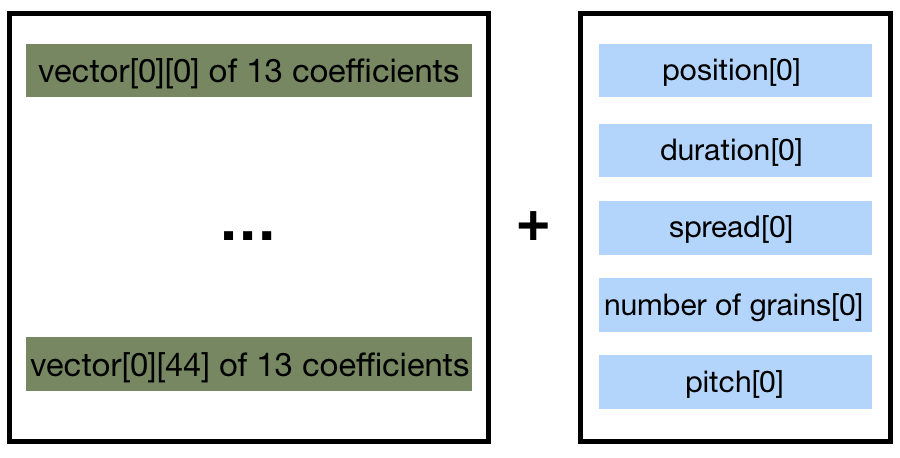
\includegraphics[width=0.8\textwidth]{images/dataset_example}
\end{figure}

Then, two arrays are created, which contain the audio analysis
results, and parameter values. In order to conveniently export these
results as .JSON files, the arrays are appended to a `Pool' data
structure from the `Essentia' library. `Pool' includes an elegant
solution for saving it's contents into a .JSON file with the help of
`YamlOutput' function, like so:

\begin{lstlisting}
  mergedMFCCs = factory.create("YamlOutput",
                                  "filename", "MFCC.json",
                                  "format", "json",
                                  "writeVersion", false);
  mergedMFCCs->input("pool").set(mergePool);

  mergePool.merge(pool, "append");
\end{lstlisting}

The resulting dataset is imported into a Python script, in order to
perform the training of different predictive models.
% maybe add example JSON output of one frame and maybe a diagram of structure

\subsection{Neural networks}

% (check if true, and quote the infamous paper - last sentence
There are many different possibilities when it comes to
the architectures and types of networks. It was shown that a
Multilayered Perceptron, as well as Long-Short Term Memory network are
both viable choices, with Bidirectional LSTMs having the best
performance\cite{yee-king_automatic_2018}.

Due to time constraints, as well as the lack of expertiese in the
field of deep learning, only two basic models were implemented. A feed
forward Multilayered Perceptron, and a Long-Short term memory
network. The popular ``Keras'' (source) library was used to create the
architectures for both of these models in Python.

Next, I detail both implementations, as well as discuss the basic
theory behind each network.  

\subsubsection{Multilayered Perceptron}
% add specific values in the paragraph about how many epochs
% etc... look at python code for this!!!!!!!!!

A Multilayer Perceptron is considered to be a ``vanilla'' neural
network. It consists of at least 3 layers of nodes - an input layer, a
hidden layer, and an output layer. The data flows only in one
direction, therefore it is often reffered to as a feedforward neural
network. A minimum architecture for such a network can be expressed
with a diagram, like so:

% change to one i made 
\begin{figure}[!h]
\caption{Minimal Multilayer Perceptron architecture}
\centering
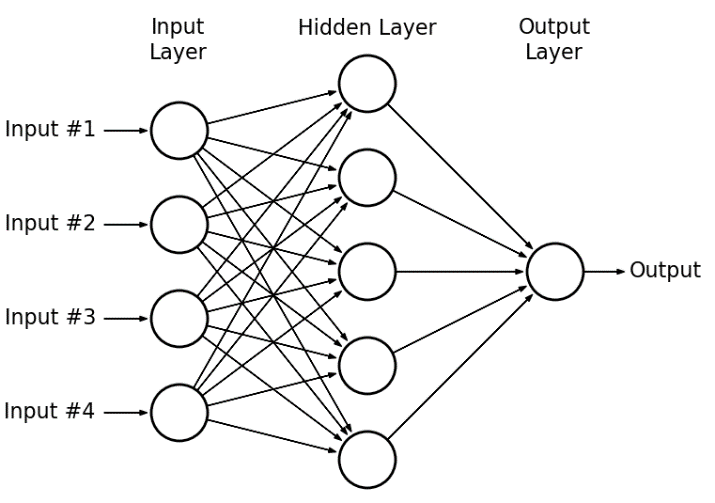
\includegraphics[width=0.8\textwidth]{images/MLP}
\end{figure}

In a regression problem, such as one cosidered in this project, the
nodes in the hidden layer(s) all use a nonlinear activation
function. Possibly the most significant historically are the two ``sigmoid''
activation function, which essentialy maps any input between the
values 0 and 1. (source?)

$y(v_i) =$tanh$(v_i)$ and $y(v_i) = (1+e^{-v_i})^{-1}$
% maybe a diagram here as well, to compare to ReLu

Today, many different actiavtion functions can be used, with the most
popular and universal being the ``ReLu'' rectifier:

$f(x) =$ max$(0, x)$
% add equation, diagram? look at james' thesis

% backpropagation explained below, how gradient descent works look at
% james' thesis to see how he decribes nn
The training of an MLP utilizes a backpropagation (sorces from wiki)
technique, which falls into the supervised learning category of
machine learning. Backpropagation is commonly used by the gradient
descent optimazation algorithm, to adjust weights of each node by
calculating the gradient of a loss function.

There is a large number of loss functions used for this purpose They
vary for different problems. For regression, the most commonly used
are ``mean squared error'' and ``mean absoulte error''.

% 2. as all nn (james) all of this is done automatically in Keras
All this is done automatically in ``Keras''.

My implementation of the Multilayer Perceptron has the following
architecture:

% graph of my net

The data was split into training and test sets, where 80\% served as
the training, with the remaining 20\% as test set.
% add code

The 45 by 13 MFCC vectors contained in the .JSON file, were imported
into Python by using the standard json library. (source), and
converted into numpy arrays, to allow further processing. Scaling of
data between 0 and 1 is also done at this stage using the
``MaxMinScalar'' from the ``sklearn'' library.
\begin{lstlisting}
import json
import numpy as np
from sklearn.preprocessing import MinMaxScaler

with open('MFCC.json') as f:
    d2 = json.load(f)

mfcc = np.array(d2["lowlevel"]["mfcc"])
scaler.fit(mfcc)
mfcc_norm = scaler.transform(mfcc)
mfcc_norm_reshaped = mfcc_norm.reshape(10000, 45, 13)
\end{lstlisting}

As seen in figure X.X, the input layer consited of 585 nodes. The
second layer of 20 nodes, the third of 15, The amount of nodes in the
output layer is equal to the number of parameters to be predicted,
which in this case is 5. The 2D input vectors were flattened before
feeding them to the hidden layers so that the entire second of MFCC
values could be fed into the network at once. This model is defined as
follows: 
% change layers values after finding the actual code used
\begin{lstlisting}
model = tf.keras.Sequential([
    layers.Flatten(input_shape=(45,13)),
    layers.Dense(585, activation='relu'),
    layers.Dense(128, activation='relu'),
    layers.Dense(64, activation='relu'),
    layers.Dense(5)])
\end{lstlisting}

% edit:
Values of the hidden layers, are arbitrary, and were decided
by experimentation with different hyperparameters. This is something
that could be drastically improved, in order to get better results
probably.

% hyperparameters
The activation function used for all hidden layers was the ``ReLu''
rectifier, and the ``Adam'' optimizer was used, with the mean absoulte
error as the loss function. This translates to ``Keras'' code like so:

In the training of an early stopping function was used to prevent
overfitting.
% code

With this in place, the network was trained for 567 (change)
epochs. The final loss function values were 0.9 for training set, and
0.12 for the test set.

% training proedure
The network was trained for X epochs, making use
of an early stopping function, to prevent overfitting. The loss
function values for training set is about 0.9 and test set 0.12.

\subsubsection{LSTM}

Leave for now, don't think I know enough to get into this business.

\section{Synthesis}
% find place for this; 
Many software based granular synthesizers exist, both in standalone
(source, source) and VST form (sources). The implementations, and
certain parameters etc. differ in each example. Nonetheless, this type
of synthesis introduces an interesting problem in the contex of
parameter prediction, which applies to any corpus based synthesis
engine. The sounds created are heavily based on the sample fed into
the synthesizer. Each parameter changes meaning significantly, once
the input sample has changed. 

Two possible solutions come to mind, when trying to overcome this
problem.

Training a model, for an instance of a granular synthesizer with a
perticular sample uploaded as the source file, therefore teaching the
``agent'' how to predict parameters for that perticular sample is one
solution. This carries some obvious disadvantages, such as the
inability to change the input samples, limiting the synthesizer to
one. To improve this approach, multiple models could be trained, on a
library of samples to give the possibility of predictions on a larger
scale.

Another, would be trying to fit some universal analysis algorithms,
that could decribe rhythym, pitch, density of sound etc. independently
of the original sample. This way any sample could be `molded' into
what would resemble the original prediction target. As described in
(METHODS-PREDICTION) section, this approach was disregarded for this
project, because of lack of evidence in literature, as well as one
failed attempt at creating such a correlation. 

Concatenative synthesis is an alternative approach to this problem. It
could be beneficial, as it would try to find `grains' as closely
resembling parts of the target as possible, and recreate it using
little parts, almost like puzzles, that the algorithm thinks
fit. However, that approach also has limitations, as it could only
recreate the target sound out of the samples stored in it's database,
therefore making the output biased. (cataRT source)

The decision of using a granular synthesiser for this program was made
based on my personal preference for this type of synthesis, and the
general lack of research focusing on corpus-based synthesis in this
domain, as mentioned in (CHAPTER 2). Even though efforts were made to
direct this problem perticularily at an instance of a granular
synthesizer, the approach used could be applied to just about any
other synthesis engine out there.

In the next sections I first explain the basic concept of granular
synthesis, and then go on to explain my own implementation, used in
this project.

\subsection{Granular Synthesis}

Describing granular synthesis in one paragraph is impossible
without cutting some edges, and leaving out many intricacies of the
technique. However, a summary of sorts, describing the main concepts
behind the algorithm will be attempted here. 

Granular synthesis is a relatively recent synthesis
technique. However, it has been theorised for decades before it could
have been implemented as a computer program. It' seed lies within 
general ideas about the nature of sound. Quantum physics has shown
that sound can be atomically reduced to physical particles (WIENER
REF). Isaac Beeckman was one of the first people to envision this
physical form of sound (Cohen 1984), arguing that sound travels
through the air as globules of sonic data.

These particles of data are imitated and magnified in this synthesis
method, and are commonly reffered to as grains, hence the
name of the technique itself. Combining these grains leads to the
creation of different sonic events.

The original research by Gabor (source), was not intended at musical
applications, until it reached the hands of Xenakis, who saw the
potential of this technique. His first trials at granular synthesis
included physically cutting magnetic tape into tiny pieces, and taping
them back together in different order.

This research extended into the realm of computers with the help of
Roads, who, after attending a seminar by Xenakis, began experimenting
with this idea at the University of XXX. First experiments of
implementing this technique took days to render a second of monophonic
sound. 

First realised real-time implementation of the granular synthesis
technique was realised in 1986, by Traux (source).

% perhaps edit this ripoff
From this point on, granular synthesis has slowly become available to
a growing number of musicians and sound artists.

% get sources from here
% The original intent of the
% process described by Gabor was to reduce the amount of data required
% to convery an audio human communication, necessitated by the low band
% width, but rising usage of telecommunication devices in the 1940s
% (Gabor 1946).
% Gabor's research came into the hands of Xenakis, who recognised a
% musical application for this work (Xenakis 1971).
% After reading an article about granular
% synthesis written by Roads in 1978, Truax began developping a way to
% create granular synthesis in real-time, first realised in 1986.


% describe process more here:
In recent implementations of granular synthesis, an audio sample is
used as the basis from which grains are extracted. Providing a
waveform for each separate grain. The grains are essentially
small snippets of the original sample, rearanged together in
different ways.

The most basic granular synthesiser requires some sort of an envelope
over the grain, grain waveform, whether generated by an oscillator or
taken from a sampled audio, and some grain spatialization. Here is a
graph representing a minimal implementation, taken from ``Microsound''
by Curtis Roads.
%graph from microsound

It is an extremely versatile method of synthesis, capable of
generating anything between pitched sounds, continous sounds, to
segmentation techniques, all dependent on 3 main parameters. Grain
envelope, grain waveform, and grain length.

\subsection{Implemnting Granular Synthesis in JUCE}
% have to mention about the ability of working on only one sample
% somewhere here...
In order to meet the goal of creating a standalone, user-facing
program, with all the functionality mentioned in (CHAPTER 1) an
original implementation of granular synthesis was made. It allowed for
the other modules to be implemented inside of the synthesizer,
cosequently making the program independent.

A possibility of creating only the audio feature extraction, and
machine learning modules, and integrating them with an external,
already existing synthesiser exists, such as done by Yee-King et
al. However this approach would clearly not allow for a creation of a
``all in one'' program, as stated in (CHAPTER 1).

The ``JUCE'' library served as the foundation for the synthesizer. It
is one of the most established libraries in the professional audio
community, being used by companies such as `Cycling 74', and `Korg'
amog others (cite website?).  On top of all things audio, it provides
a convenient way of creating a graphical user interface, which was an
important part of this project.  Thanks to `JUCE', the implementation
was kept minimal, and elegant.

Even though the concept of granular sythesis is very difficult, the
implementation here is kept fairly minimal, to restiric the amount of
dimensions, reducing learning time for the neural networks, and
consequently minimizing the time needed to create an appropriately
sized dataset.

In reponse to these requirements only 6 adjustable parameters were
implemented.

Below i go through all the parameters, and basic concepts of the
implementation of granular synthesis in code.

General architecture is based on these programs also implemented in
JUCE: links to github.

% explain the grain vector
All the functionality for grains is contained in the "GrainStream" class, 
defined in the "Grain.cpp" file (code included in the appendicies).

\subsubsection{Loading audio files}
% add that only wav files accepted
% maybe add a picture here to add visual aid for explenation

Loading audio files is the first step to acheive any output from the
synthesizer, as it relies on sourcing waveforms for each grain from
preexisting audio. Handling of this behaviour is made easy thanks to
the ``JUCE'' framework: 
\begin{lstlisting}
  void GrainStream::setAudioSource(AudioFormatReader& newAudioFile)
  {
    int length = static_cast<int>(newAudioFile.lengthInSamples);

    //update grain parameters
    this->fileSize = length;
    this->samplingRate = static_cast<int>(newAudioFile.sampleRate);

    //clear the audio source and read new WAV
    this->AudioSourceBuffer.reset(new
                                     AudioSampleBuffer(newAudioFile.numChannels, length));
    newAudioFile.read(this->AudioSourceBuffer.get(), 0, length, 0,
                        true, true);
  }
\end{lstlisting}

``JUCE::AudioFormatReader'' and ``JUCE::AudioSourceBuffer'' classes
are used to handle this behaviour. The length of the sample, as well
as it's sampling rate are also read here, and used to update global
values. Used for different purposes, which will all be detailed later
in this chapter.

\subsubsection{Grain creation}
% code for grain creation

First, let's define what a grain is in the program. A single grain is
defined as a ``struct'':
\begin{lstlisting}
    // this contains data about a specific grain inside the grain stream
    struct oneGrain
    {
        double grainDataCurrentSample[2] = {0.0, 0.0};
        
        int grainDataStartPosition = 0;       // starting sample for a specific grain
        int grainDataEndPosition = 0;            // ending sample of a specific grain
        
        double grainDataPitchScalar = 1.0f;    // scalar value for randomized pitch offset
        double grainDataGainScalar = 1.0f;      // scalar value for rand gain offset
        
        bool grainDataIsFinished = true;       // boolean whether grain needs to be replayed
        
        juce::ADSR adsr;
        juce::ADSR::Parameters adsrParams;
        
        bool inRelease = true;
    };
\end{lstlisting}

We can see that each grain has two doubles for one sample on each
channel. It has a start and end position, as well as two scalars - one
for pitch and one for the grain of each grain. One grain also contains
a bool, to determine is a specific grain is currently playing. As well
as an ``adsr'' envelope, defined with the ``JUCE::ADSR'' class, and
another bool to determine whether the envelop is in the state of
release.

Grains are created by specifing samples from the audio input (.WAV
file loaded before synthesis) to be loaded into the ``oneGrain''
struct.
\begin{lstlisting}
void MainComponent::getNextAudioBlock (const AudioSourceChannelInfo& bufferToFill)
{
    if (grainStream.grainStreamIsActive && record == false)
    {
        for (auto channel = 0; channel < bufferToFill.buffer->getNumChannels(); ++channel)
        {
            // get a pointer to the start sample in the buffer for this audio output channel
            auto* buffer = bufferToFill.buffer->getWritePointer(channel,
                                                                      bufferToFill.startSample);

            // fill each grain struct with samples 
            for (auto sample = 0; sample < bufferToFill.numSamples; ++sample)
            {
                buffer[sample] = grainStream.createGrain(channel);
            }
        }
     }
}
\end{lstlisting}

The ``createGrain'' function above is determining from where exactly
to take those samples, based on the parameters set by GUI dials. The
parameters will be explained separately in the next sections.
% code for createGrain here, but first have to clean it up.

\subsubsection{Position}

First parameter users have direct access to is the position in an
audio file, from which grains will be generated. Value of this
parameter is determined by the ``FilePos'' dial.

It's value serves as a parameter to the `setFilePosition' function, which
in turn communicates the starting position for each grain with the
use of ``filePosition'' integer.

% It was required to subtract 1 from the dial's value, because...XXX ??????

The following code is responsible for
this task:
\begin{lstlisting}
  void GrainStream::setFilePosition(int startingSample)
  {
    this->filePosition = startingSample - 1;
  }
\end{lstlisting}

This value is then sent to the SETUP GRAIN function, where the
``grainDataStartPosition'' integer for each grain is set, consequently
making the grain spawn in that position.
\begin{lstlisting}
grain.grainDataStartPosition = this->filePosition;
\end{lstlisting}

\subsubsection{Grain Size}

Grain size parameter is and can be defined as the difference between
the start and end position of the grain, in other words delta.

$\Delta y = y_2 - y_1$

Where $y_2$ is the end position, and $y_2$ is the start position of
the grain. This delta is calculated by deviding the grain size in
milliseconds (it's duration), by 1000 and multiplying it by the
current sampling rate, in order to convert that value to samples. The
end position is then calculated by simply adding the delta to the
start position.

The size of each grain varies between the minimum of 10ms and maximum
of 1 second. It can be easily set using the Grain Size GUI dial. Value
of the dial serves as a parameter to the `setDuration' function:
\begin{lstlisting}
  void GrainStream::setDuration(int duration)
  {
    //update duration and compute sampleDelta
    this->durationOfStream = duration;
    this->sampleDelta = static_cast<int>(this->samplingRate *
    (duration/1000.0f));

    for (oneGrain grain : grains)
    {
      grain.grainDataEndPosition = grain.grainDataEndPosition +
      this->sampleDelta;

      if (grain.grainDataEndPosition >= this->fileSize)
          grain.grainDataEndPosition = (this->fileSize - 1);
    }
  }
\end{lstlisting}

Simple but effective error handling is then implemented, by ensuring
that the end position of a grain will never be bigger than the length
of the sample.

\subsubsection{Spread}

The spread parameter is determining the size of an area around the
file position, from which grains will be spawned. In other words, it
randomizes the starting position for each grain, within a certain
range. 

This range is determined by the spread parameter itself, which in code
is represented as ``filePositionOffset''. 
\begin{lstlisting}
  Random rand = Random();

  // Randomize the Starting Sample
  grain.grainDataStartPosition = rand.nextInt(Range<int>
                                              (this->filePosition - filePositionOffset,
                                               this->filePosition + filePositionOffset));

  // Prevent samples from being outside of file range 
  if (grain.grainDataStartPosition < 0)
      grain.grainDataStartPosition = 0;
  else if (grain.grainDataStartPosition >= this->fileSize)
      grain.grainDataStartPosition = (this->fileSize - 1);
\end{lstlisting}

Again, the JUCE:Random class is used as the pseudorandom number
generator. For each grain, the code above generates a new start
position, in the range of current position plus and minus the offset
determined by the spread parameter.

To give an example, let's assume that the position is set to 10000
samples, which would correspond to approximately 4 seconds into the
file, assuming a samapling rate of 44,1kH. With the spread at 0, each
consequtive grain would start at exactly 10000 samples, play for it's
duration, and die, creating space for another grain to be spawned,
again at the starting position of 1000 samples. Once the dial has a
value bigger than 0, a random number is generated in the appropriate
range, consequently creating a new start position for each grain. With
a spread value of 200, each grain's new start position would equal to
some number in the range of 9800 and 10200 samples.

This allows for each grain to have independent starting positions,
creating a more interesting clusters, that do not sound so repetative
and static.

The case of the spread parameter being zero:
\begin{lstlisting}
if (filePositionOffset == 0 || (this->filePosition - filePositionOffset) <=0)
grain.grainDataStartPosition = this->filePosition;
\end{lstlisting}

\subsubsection{Number of active grains}
\begin{lstlisting}
// vector containing grains 
vector<oneGrain> grains;
\end{lstlisting}

The amount of grains available is predetermined arbitrarily by the
range of values available within the parameter dial. These values are
set to a range between 1 and 10, meaning that the 2D vector ``grains''
can contain up to 10 ``oneGrain'' structures, as defined in section 3.3.2.2. 

The GUI dial value is sent directly into the function shown below, as
the ``size'' parameter, which then decides whether to add or remove
grains from the vector.
\begin{lstlisting}
void GrainStream::setStreamSize(int size)
{
    if (size > this->grainStreamSize)
        addGrainsToStream(size - this->grainStreamSize);
    else if (size < this->grainStreamSize)
        removeGrainsFromStream(this->grainStreamSize - size);
}
\end{lstlisting}

Adding grains to the stream is done by simply adding a grain data
structure to the 2D vector containing all the grains; the stream of
grains, defined above.
\begin{lstlisting}
void GrainStream::addGrainsToStream(int count)
{
    for (int i = 0; i < count; i++)
    {
        // append a grain the stream
        grains.push_back(oneGrain());
    }
    
    // update stream size
    this->grainStreamSize += count;
}
\end{lstlisting}

Following the same principle, the removal of grains is done like so:
\begin{lstlisting}
void GrainStream::removeGrainsFromStream(int count)
{
    for (int i = 0; i < count; i++)
        grains.pop_back();
    
    this->grainStreamSize -= count;
}
\end{lstlisting}

Because of this, the interaction is kept quite simple, and the size
can be decided with the use of only one dial. If the value of the dial
if bigger than current size of the stream, we remove grains to match
the value. Conversly, if the dial value is smaller, we add grains to
the 2D vector `grains'.

\subsubsection{Pitch}
% figure this out properly if enough time!
Each grain, as defined in the `OneGrain' struct defined above, has a
variable called grainDataPitchScalar, responsible for changing the
pitch of grains independently. In the spirit of simplicity, however,
in this perticular implementation, the pitch scalar is kept global,
with the possibility of extension.

It is binded to the Pitch dial visible in the GUI, which changes the
`pitchOffsetForOneGrain' variable, which is then sent to the :

% CODE

% this part of the code is probably fucked up hahahhaahahahahahha :(
The grain.grainDataPitchScalar can therefore only have values between
THIS and THAT, consequently either speeding up or slowing down the
playback of each grain, and affecting the pitch.

\subsubsection{Global gain}
The global gain of the signal is simply controlled by the globalGain
variable, which is used for scaling each individual sample sent to the
audio buffer like so:
\begin{lstlisting}
  sample *= static_cast<float>(globalGain)
\end{lstlisting}

The globalGain variable is directly controlled with the global gain
dial in the GUI.

\subsubsection{Sound output}

The sound output is mostly handled by the JUCE library, with the use
of the provided `getNextAudioBlock' function. The audio block, or
buffer is being filled with samples determined in the Grain class,
more specifically, in the `createGrain' function contained within that
class:

%code here

All the functionality needed to determine all the previously mentioned
parameters is  here. What is being returned is samples, one by one
with which to fill both channels of the buffer.

% (where do the grains come from)(how does the
% behaviour change depending on the sample)

%maybe add stuff from microsound about the parameters, and how they
%influence the sound.
%
%also, maybe add how the personal preference for the granular sound
%influenced this area of production.

\section{Integration}

Some form of communication between all 3 main modules had to be
implemented, in order to achieve real-time, or near real-time
results. Whatever sound chosen to serve as the target for prediction
has to first be analysed, in order to extract relevant MFCC. Then,
these values have to somehow be sent into the neural network model, to
get a prediction of parameters, for these MFCC. Then, these results
have to be assigned to the actual parameters in the synthesizer.

Different approaches were considered for handling this communication.

During the first few iterations of the project, starting with the
first prototype, OSC messages were used to send audio analysis values
to Python, predict parameters there, and send the predictions back to
C++.

This process however, was not optimal. It was relatively slow, not
efficient, and required two separate programs to be running in order
to give basic functionality.

The most intuitive way of doing that in my eyes, was to somehow
integrate this entire process into the synthesis program, so that
these processes could be easily accessed, and done within one window,
with as much simplicity to the process as possible.

% here are some different ways of doing that (integration of python
% with C++)

During the later stages of the production, I have found a satisfying
solution to this problem. The ``Frugally Deep'' library (source). It
allows for converting a model saved in ``Keras'' as a .json file, into
XXX, and allow for it's usage directly in the C++ code. Consequently,
allowing for real time predictions.

Consequently, the model in Keras was saved after training with like so:
%CODE

With the toolset supplied by the `Frugally Deep' library, it was then
converted into XXX like so:
%CODE

% this is how data was converted
% this is how it was passed to the model
The data had to be sent into the model, and for that i'm using this thing:

% this is how it was scaled
the model was trained on scaled data, therefore to get the right
predictions we have to scale it down in c++ also

% this is how it is retrieved from the model
another thing is that we have to scale it back up to the right
parameter ranges, this is done with the values from MinMaxScaler
copied from python

% conclusion
As seen above, with the file converted, only a few lines of code were
needed to make use of the model directly in the C++ synthesis program,
creating a standalone application, silmultaniously allowing for much
quicker and simpler performance, without the need of any additional
software running.


%What belongs in the "methods" section of a scientific paper?
%
%    Information to allow the reader to assess the believability of your results.
%    Information needed by another researcher to replicate your experiment.
%    Description of your materials, procedure, theory.
%    Calculations, technique, procedure, equipment, and calibration plots. 
%    Limitations, assumptions, and range of validity.
%    Desciption of your analystical methods, including reference to any specialized statistical software. 
%
%The methods section should answering the following questions and caveats: 
%
%    Could one accurately replicate the study (for example, all of the optional and adjustable parameters on any sensors or instruments that were used to acquire the data)?
%    Could another researcher accurately find and reoccupy the sampling stations or track lines?
%    Is there enough information provided about any instruments used so that a functionally equivalent instrument could be used to repeat the experiment?
%    If the data are in the public domain, could another researcher lay his or her hands on the identical data set?
%    Could one replicate any laboratory analyses that were used? 
%    Could one replicate any statistical analyses?
%    Could another researcher approximately replicate the key algorithms of any computer software?
%
%Citations in this section should be limited to data sources and references of where to find more complete descriptions of procedures.
%Do not include descriptions of results. 


%%% Local Variables:
%%% mode: latex
%%% TeX-master: "dissertation"
%%% End:


\chapter{Results and Analysis}
%no interpretation of results!

As stated in \autoref{intro}, the success of this project is dependent
on three objectives, Firstly, the tool built has to be somewhat
helpful to artists in creating new sounds. It will ideally challenge
the interaction between a user, and presets, as a starting point to
synthesis. Lastly, the results of parameter predictions must in fact
bear some resemblance to the target sound, and be more than a mere
randomisation of parameters.

As it is a user centred program, the users must feel like it indeed
generates sounds that they find similar to the supplied input, and not
less importantly, that the program is interesting to them, that an
interaction it commences has some value, and to put it simply, it is
fun to use. Additionally, the software must be intuitive, and easy to
use, and ideally the user interface should not bring any confusion.

\section{Methodologies}

Firstly, it has to be ensured that all parts of the system are working
correctly and as expected. In order to do that, some quantitative
evaluation has to be done on each module of the system.

Namely, the correctness of extracted MFCC from the signal has to be
confirmed. The synthesizer has to work as expected. The neural
networks implemented have to give predictions in expected ranges, and
finally the sounds achieved through them have to be evaluated to
determine if they are if fact similar to the targets.

Qualitative evaluation had to be done to determine if users confirm
the results of quantitative evaluation at least to some extent, as well
as to determine if it achieves objectives \#1 and \#2. More
specifically, how easy the user experience is, unrelated to the
quality of predictions.

The quantitative evaluation was conducted by comparing spectra of
target, and predicted sound. Both generated with the instrument
itself, as well as with input form the microphone.to provide a more
realistic scenario. Euclidean distance between MFCCs was measured, as
a metric of sound similarity.

The qualitative user testing, was made up of interviews, and a
questionnaire. The users were briefly introduced to the concept of the
program, and given most basic usage instructions. During the testing,
users were allowed to comment freely, and after the session they had
to fill in a questionnaire. This has allowed for immediate feedback,
as well as a possibility to reflect upon the experience, and the
ability to share those reflections later.  Interviews were recorded,
which allowed for immediate feedback, and the opportunity to
investigate them later.

\section{Audio descriptors}
% audio features - correct ?
To determine the correctness of MFCC implementation, a simple test of
the sizes of MFCC vectors is suffice. If the number of coefficients
for one frame is equal to the expected value, and if the number of
MFCC vectors in a second of sound is of expected length, then the
features obtained should be correct.

Looking at the implementation of the MFCC algorithm, within
``Essentia's'' documentation, it is clear that the length of each
vector containing MFCCs for one frame should be 13. Meaning that
exactly 13 coefficient should be extracted for each frame.

Below, we can see that, in fact the length of one MFCC vector is as expected.

% picture of cout of mfcc vector 

In turn, in order to check the validity of the legth of the vector
containing MFCCs for one second of sound, we have to dive deeper into
parameters for each consecutive algorithm computed on the signal
before MFCC.

Assuming that the length of one frame, onto which our one second of
sound should be cut into is 2048 samples, with a hopsize of 1024
samples, we should end up with 43.066 frames at the sample rate of
44.1kHz. This is of course impossible, and the most common way of
dealing with such a problem is zero-padding. ``FrameCutter'' does this
automatically and is zero-padding incomplete frames, or frames that
are going past the end of the buffer. Therefore we end up with exactly
45 frames, or MFCC vectors per second of sound. The 44th frame is
zero-padded. Noise is added to the 45th frame for equal extraction, as
in accordance to the ``siletFrames'' parameter of the ``FrameCutter''
algorithm.

Here we can see the output of the 2D vector containg all MFCCs for a
one second buffer.

We can see, that the implementation of the MFCC algorithm is therefore
sound, as we get exactly 45 vectors each containing 13 MFCCs, as expected. 

\section{Granular Synthesis}
The evaluation of the synthesis method is perhaps the most
straightforward. All that has to be made sure of, is that all
functions are working correctly, and each parameter does what it is
supposed to.

This is mostly ensured by listening evaluation conducted by myself,
and testing of each function by using the synthesizer.

%% do all functions work, is the behaviour correct, as I would expect
%% it?

% perhaps go into more detail here, with some form of confirmation of
% cout in the program?
% add shit here only if really desperate for words.

\section{Neural Networks}
% nns - correct ?
%% loss function graphs ?

In turn, the implementation of neural networks is possibly the part of
the project which will have most obvious influence over the final
results, and consequently this will decide whether predicted sounds
are in fact similar, and how similar to the targets.

Other aspects of course also have influence over this, however it
seems like neural networks will definitely determine the biggest
aspect of this problem. If they fail, the predictions will be
completely unrelated.

% make sure dataset is corrrect
% make sure loss is going down
% put in the graph of the loss function going down

The thing that has to be taken care of first, is the dataset used for
training. In order to ensure, that the data is coming into the model
as expected, the numpy arrays are simply printed to the console.

We can see that the loss function is lowering in value, until the
500th epoch here, and after that stays relatively stable, leading to
overfitting. 

\section{Sound similarity}
% microphone vs. synthesis output - mas importante

\subsection{Quantitative evaluation}

In order to determine, if predictions made by the program are viable,
and to judge how well they work, quantitative testing was performed in
form of measuring a Euclidean distance between target and predicted
MFCCs.

First, the testing was done on target sounds created with the
granulator itself. Meaning, that technically, the sounds should be
reproducible exactly, because they were made with the same instrument
we are trying to recreate it on. I now describe the process for one
iteration of such testing, and put results of one 10 instances in a
XXX table.

First, random parameter values were set, by using the function for
random parameter walkthrough. Once the parameters were set, one second
recording of the synthesizer's output was recorder into a buffer, on
which MFCCs were extracted. These values were saved, for future
access. Then, based on those MFCCs, a prediction was made using the
``Keras'' model, which automatically set values of all parameters
based on it's results. Then that was recorded into a buffer, and MFCCs
were extracted. With these two vectors of MFCCs, a Euclidean distance
was calculated between them, using the ``scikit learn'' library.

% The reason behind comparing the Euclidean distance rather than the
% parameters themeselves was the fact that as a matter of fact the
% parameter values predicted can differ quite largely from the target
% values, as certain sounds are likely possible to achieve using more
% than one parameter setting. (source) into a buffer, and MFCCs
% were extracted.

This entire process was later repeated with input from the microphone,
instead of output from the synthesiser, to determine how the model
behaves on data it has never seen before.

The reason behind comparing the Euclidean distance rather than the
parameters themeselves was the fact that as a matter of fact the
parameter values predicted can differ quite largely from the target
values, as certain sounds are likely possible to achieve using more
than one parameter setting. (source)



plan for this testing:

set some parameter values with a random button
record a second into a buffer
save MFCCs
predict parameter values
record prediction into the buffer
save MFCCs

calculate euclidean distance between them in python

do that same thing with microphone input

additionally try to save them so that mfcc's can be taken. either into
ableton (easiest) or write to a file (maybe time consuming)

%%% mfcc euclidean distance
\subsubsection{MFCCs distance}
% how it was measured
% show results on for example 10 predictions in a table
% describe the results of this - succesfull?

%%% fft images
\subsubsection{Spectra}
% pictures and descriptions

%%% random button vs prediction
\subsubsection{Random button vs. predictions}
% implement random button...

\subsection{Qualitative evaluation}

With the the technical assessment established, the testing could
proceed ``into the real'' world, where it's validity among users would
be tested. I believe, that with this software the assessment of how
similar the predictions are to the input sounds is equally important
as the quantitative results.

Additionally, their enjoyment of the experience, as well as their
overall impressions are an important factor in the assessment of
success of this project. During the tests, I was also hoping to gain
feedback about things that I have overlooked during the production,
and suggested ways of improving the user experience. 

Therefore, several testing sessions with potential users of this
software were conducted. All participants had some background in
programming synthesizers, as well as background in music
production. In order to ensure that they would somewhat resemble the
user group this software is aimed at.
% change this, it's not really aimed at anyone

The session consisted of a brief explanation of what the project is
meant to do, and a basic user guide, about how to use it. More
specifically an explanation of how the ``record'' and ``predict''
buttons work. However, the information given was fairly minimal, and
is only what was needed to introduce participant to this new concept
of interaction. This was done in hope to later access the easiness of
use, once the basic idea of interaction was established.

% some summary of the interviews here ?

After the session, participants were shown a form to fill in,
summarising their experience, and looking to establish a translation
of their experience into quantitative data.

\subsubsection{Results}
% graphs etc.

% here about users
%------------------------
% all respondents reporter a fairly good ability to program
% synthesizers
% they reported stumbling upon these problems
% most reported that their ability comes from these things

%here talk about feedback about the program
%-------------------------------------------
% the usefulness of the tool was rated quite high
% alternative to presets - yes
% how similar were the sounds predicted?
% ease of use?

% suggested stuff and additional feedback from users
%------------------------------------------------------
% 



\section{User experience}
% user experience
%% talk about the interviews somehow
%% include results from the form about the ease of use and include longer feedback


%%% Local Variables:
%%% mode: latex
%%% TeX-master: "dissertation"
%%% End:


\chapter{Discussion}
\label{chapterlabel5}
\section{Summary of Findings}
\section{Evaluation}
\section{Future Work}

Start with a few sentences that summarize the most important results. The discussion section should be a brief essay in itself, answering the following questions and caveats: 

    What are the major patterns in the observations? (Refer to spatial and temporal variations.)
    What are the relationships, trends and generalizations among the results?
    What are the exceptions to these patterns or generalizations?
    What are the likely causes (mechanisms) underlying these patterns resulting predictions?
    Is there agreement or disagreement with previous work?
    Interpret results in terms of background laid out in the introduction - what is the relationship of the present results to the original question?
    What is the implication of the present results for other unanswered questions in earth sciences, ecology, environmental policy, etc....?
    Multiple hypotheses: There are usually several possible explanations for results. Be careful to consider all of these rather than simply pushing your favorite one. If you can eliminate all but one, that is great, but often that is not possible with the data in hand. In that case you should give even treatment to the remaining possibilities, and try to indicate ways in which future work may lead to their discrimination.
    Avoid bandwagons: A special case of the above. Avoid jumping a currently fashionable point of view unless your results really do strongly support them. 
    What are the things we now know or understand that we didn't know or understand before the present work?
    Include the evidence or line of reasoning supporting each interpretation.
    What is the significance of the present results: why should we care? 

This section should be rich in references to similar work and background needed to interpret results. However, interpretation/discussion section(s) are often too long and verbose. Is there material that does not contribute to one of the elements listed above? If so, this may be material that you will want to consider deleting or moving. Break up the section into logical segments by using subheads. 

\chapter{Conclusion}
\label{chapterlabel6}


    What is the strongest and most important statement that you can make from your observations? 
    If you met the reader at a meeting six months from now, what do you want them to remember about your paper? 
    Refer back to problem posed, and describe the conclusions that you reached from carrying out this investigation, summarize new observations, new interpretations, and new insights that have resulted from the present work.
    Include the broader implications of your results. 
    Do not repeat word for word the abstract, introduction or discussion.



\appendix
\section{Title of Appendix A}

\printbibliography

\end{document}
